
\de{ĐỀ THI GIỮA HỌC KỲ I NĂM HỌC 2022-2023}{THPT Marie Curie}

%%%% Bài 1
\begin{bt}%[0T1K3-2]%[Dự án đề kiểm tra GHKI NH22-23 - Thành Đức Trung]%[THPT Marie Curie - Hồ Chí Minh]
Cho tập hợp $A=\{-2 ; 3 ; 5\}$ và tập hợp $B=\{-1 ; 2 ; 4\}$. Xác định các tập hợp sau:
\begin{enumerate}
\item  $A \cap B$.
\item $A\setminus B$.
\end{enumerate}
\loigiai{
\begin{enumerate}
\item 	Ta có $A \cap B=\varnothing$.
\item $A\setminus B=\{-2;3;5\}$.	
\end{enumerate}
}
\end{bt}

%%%% Bài 2
\begin{bt}%[0T1B3-2]%[Dự án đề kiểm tra GHKI NH22-23 - Thành Đức Trung]%[THPT Marie Curie - Hồ Chí Minh]
Cho tập hợp $A=\left(-5;3\right]$ và tập hợp $B=\left(-\infty;3\right)$. Xác định các tập hợp sau
\begin{enumerate}
\item $A\cap B$.
\item $A\cup B$.
\item $A\setminus B$.
\item $B\setminus A$.
\end{enumerate}
\loigiai{
\begin{enumerate}
\item $A\cap B=\left( -5;3\right)$.
\item $A\cup B=\left(-\infty;3\right]$.
\item $A\setminus B=\{3\}$.
\item $B\setminus A=\left(-\infty;-5\right]$.
\end{enumerate}
}
\end{bt}

%%%% Bài 3
\begin{bt}%[0T1B3-3]%[Dự án đề kiểm tra GHKI NH22-23 - Thành Đức Trung]%[THPT Marie Curie - Hồ Chí Minh]
Câu lạc bộ thể thao của trường Marie Curie có môn Bóng đá và Câu lông. Trong câu lạc bộ này có tất cả $35$ học sinh tham gia, trong đó có $25$ học sinh chơi bóng đá và $20$ học sinh chơi cầu lông.
\begin{enumerate}
\item Dùng biểu đồ Ven để biểu diễn các tập hợp học sinh tham gia câu lạc bộ thể thao.
\item Hỏi câu lạc bộ thể thao có bao nhiêu học sinh chơi cả hai môn, bao nhiêu học sinh chỉ chơi một môn?
\end{enumerate}
\loigiai{
\begin{enumerate}
\item Biểu đồ Ven
\begin{center}
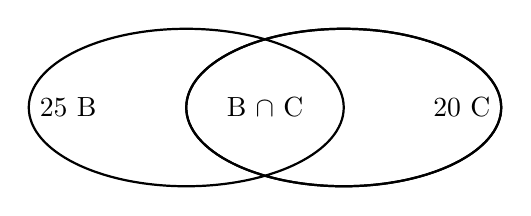
\begin{tikzpicture}[>=stealth, line join=round, line cap = round, thick]
\coordinate (A) at (0,1);
\coordinate (B) at (-7,1);
\coordinate (C) at (0,-3);
\coordinate (D) at (-7,-3);
\coordinate  (E) at (-4.5,-1);
\coordinate (F) at (-2.5,-1);
\fill[white] (-4.5,-1) ellipse ({2} and {1}) (-2.5,-1) ellipse ({2} and {1});
\draw (-6,-1)node[]{$25$ B};
\draw (-1,-1)node[]{$20$ C};
\draw (-3.5,-1)node[]{B $\cap$ C};
\foreach \x in {E,F} \draw (\x) ellipse ({2} and {1}) (-2.5,-1) ellipse ({2} and {1});
\end{tikzpicture}
\end{center}
\item 	Số học sinh chơi cả hai môn là $25+20-35=10$.\\
Số học sinh chỉ chơi đá bóng là $25-10=15$.\\
Số học sinh chỉ chơi cầu lông là $20-10=10$.
\end{enumerate}	
}
\end{bt}

%%%% Bài 4
\begin{bt}%[0T4B2-1]%[Dự án đề kiểm tra GHKI NH22-23 - Thành Đức Trung]%[THPT Marie Curie - Hồ Chí Minh]
Cho $\triangle ABC$ có $AB=2$, $AC=2 \sqrt{7}$ và $BC=4$. Tính số đo góc lớn nhất của $\triangle A B C$. (Lấy kết quả làm tròn chính xác đến phút).
\loigiai{
Do $AC>BC>AB$ nên tam giác $ABC$ có góc $\widehat{ABC}$ có số đo lớn nhất. Ta có
\[\cos B=\dfrac{AB^2+BC^2-AC^2}{2\cdot AB\cdot BC}=\dfrac{4+16-28}{16}=-\dfrac{1}{2}.\]
Suy ra $B=120^\circ$.
}
\end{bt}

%%%% Bài 5
\begin{bt}%[0T4B2-1]%[Dự án đề kiểm tra GHKI NH22-23 - Thành Đức Trung]%[THPT Marie Curie - Hồ Chí Minh]
Cho $\triangle ABC$ có $BC=7 \mathrm{~cm}$, $AC=8 \mathrm{~cm}$, $AB=6 \mathrm{~cm}$. Tính diện tích $\triangle ABC$ và bán kính $R$ của đường tròn ngoại tiếp $\triangle ABC$. (Lấy kết quả làm tròn chính xác $2$ chữ số thập phân sau dấu phẩy).
\loigiai{
Ta có $p=\dfrac{AB+BC+AC}{2}=\dfrac{6+7+8}{2}=\dfrac{21}{2}$.\\
Diện tích của tam giác $ABC$ là
\begin{eqnarray*}
S&=&\sqrt{p(p-AB)(p-BC)(p-AC)}\\
&=&\sqrt{\dfrac{21}{2}\left(\dfrac{21}{2}-6\right)\left(\dfrac{21}{2}-7\right)\left(\dfrac{21}{2}-8\right)}\\
&=&\dfrac{21\sqrt{15}}{4}\approx 20{,}33 \mathrm{~cm}^2.
\end{eqnarray*}
\noindent 
Bán kính đường tròn ngoại tiếp $\triangle ABC$ là
\[R=\dfrac{AB\cdot AC\cdot BC}{4S}=\dfrac{6\cdot 8\cdot 7}{21\sqrt{15}}=\dfrac{16\sqrt{15}}{15}\approx 4{,}13\mathrm{~cm}.\]
}
\end{bt}

%%%% Bài 6
\begin{bt}%[0T4T3-1]%[Dự án đề kiểm tra GHKI NH22-23 - Thành Đức Trung]%[THPT Marie Curie - Hồ Chí Minh]
Từ hai vị trí $A$ và $B$ của một tòa nhà, người ta quan sát đỉnh $C$ của một ngọn núi. Biết rằng độ cao của tòa nhà là $70$ m, phương nhìn $AC$ tạo với phương nằm ngang góc $30^{\circ}$, phương nhìn $BC$ tạo với phương nằm ngang góc $15^{\circ}$.
\begin{center}
\begin{tikzpicture}[xscale=.7,yscale=0.4, font=\footnotesize, line join=round, >=stealth]
\coordinate (O) at (0,0);
\coordinate[label=below:$A$] (A) at (2.2,0);
\coordinate[label=above left:$B$] (B) at (2.2,7);
\coordinate[label=above left:$C$] (C) at (11.27,13.13);
\coordinate (D) at (11.27,7);
\coordinate[label=below:$H$] (E) at (11.27,0);
\coordinate[label=right:$70$m] (I) at ($(A)!0.5!(B)$);
\coordinate[label=above left:$15^\circ$] () at (5,7);
\coordinate[label=above right:$30^\circ$] () at (3,0);
\draw[dashed](B)--(D);
\draw (A)--(C) (B)--(C) (A)--(E)--(C);
\def\nhathap{6} %so tang nha thap
\def\dai{1} %chieu dai 1 khoi
\def\cao{1} %chieu cao 1 khoi
\newcommand{\xaynha}[2]{
\draw[very thick] (#1,#2)rectangle(#1+\dai,#2+\cao);
\draw[very thick,fill=black] (#1,#2)rectangle(#1+\dai,#2+0.25*\cao);
\draw[very thick] (#1+0.2*\dai,#2+0.25*\cao)rectangle(#1+0.8*\dai,#2+0.9*\cao); 
}
%Xay nha thap
\foreach \j in {0,...,\nhathap}{
\foreach \i in {0,1}{
\xaynha{\i*1.1}{\j*\cao}	} 	}
\fill [black!30]plot [smooth ] coordinates{(6.64,0)(7.36,3.91) (7.96,5.47) (8.28,4.92) (8.63,4.77)(8.84,3.99) (9.47,5.08) (9.87,7.42)(10.4,8.36)(10.37,9.77)(11.27,13.13)(11.93,12.11)(11.83,10.55)(12.44,9.14)(12.91,6.33)(12.75,4.77)(13.94,0.7)(13.78,0)};
\draw pic[draw,blue,angle radius=5mm] {angle = D--B--C}; 
\draw pic[draw,blue,angle radius=5mm] {angle = E--A--C}; 
\end{tikzpicture}
\end{center}
\begin{enumerate}
\item Tính số đo góc $\widehat{ACB}$. (Lấy kết quả làm tròn chính xác đến phút).
\item Tính độ cao của ngọn núi so với mặt đất? (Lấy kết quả làm tròn chính xác $2$ chữ số thập phân sau dấu phẩy).
\end{enumerate}
\loigiai{
\begin{enumerate}
\item Ta có $\widehat{ACB}=180^\circ-\left(105^\circ+60^\circ\right)=15^\circ$.
\item Áp dụng định lí sin vào tam giác $ABC$ ta có \[\dfrac{70}{\sin 15^\circ}=\dfrac{AC}{\sin 105^\circ} \Rightarrow AC=70\cdot \dfrac{\sin 105^\circ}{\sin 15^\circ}=70\left(2+\sqrt{3}\right).\]
Xét tam giác vuông $AHC$, ta có $CH=AC\cdot \sin 30^\circ=35\left(2+\sqrt{3}\right)\approx 130{,}62$ m.
\end{enumerate}
}
\end{bt}

%%%% Bài 7
\begin{bt}%[0T2T2-3]%[Dự án đề kiểm tra GHKI NH22-23 - Thành Đức Trung]%[THPT Marie Curie - Hồ Chí Minh]
Cơ sở $A$ dự định dùng hai nguyên liệu là mía và củ cải để sản xuất ít nhất 140kg đường cát vàng và $30 \mathrm{~kg}$ đường cát trắng. Từ $1$ tạ mía giá $500$ nghìn đồng có thể sản xuất được $20 \mathrm{~kg}$ đường cát vàng và $2 \mathrm{~kg}$ đường cát trắng. Từ $1$ tạ củ cải giá $400$ nghìn đồng có thể sản xuất được $10 \mathrm{~kg}$ đường cát vàng và $5 \mathrm{~kg}$ đường cát trắng. Công ty cung cấp nguyên liệu cho cơ sở $\mathrm{A}$ chỉ còn $10$ tạ mía và $9$ tạ củ cải. Gọi số tạ mía cần dùng là $x$ và số tạ củ cải cần dùng là $y$.
\begin{enumerate}
\item  Hãy thiết lâp điều kiện cho $x$.
\item Hãy thiết lâp điều kiện cho $y$.
\item Hãy thiết lâp điều kiện về lượng đường cát vàng được sản xuất từ mía và củ cải.
\item Hãy thiết lập điều kiện về lượng đường cát trắng được sản xuất từ mía và củ cải.
\item Biểu diễn miền nghiệm của hệ bất phương trình thỏa mãn các ý a, b, c, d. Kết luận về miền nghiệm.
\item Hỏi nhà máy phải mua bao nhiêu nguyên liệu mỗi loại để chi phí mua là ít nhất?
\end{enumerate}
\loigiai{
\begin{enumerate}
\item 	Ta có $0\le x\le 10$.
\item 	Ta có $0\le y\le 9$.
\item  Ta có $20x+10y\le 140 \Leftrightarrow 2x+y\ge 14$.
\item  Ta có $2x+5y\ge 30$.
\item Ta có hệ bất phương trình sau $\heva{&0\le x\le 10\\& 0\le y\le 9\\&2x+y\ge 14\\&2x+5y\ge 30.}$
\begin{center}
\begin{tikzpicture}[scale=0.75,line join=round, line cap=round,>=stealth,thick]
\begin{scope}
\clip (-3,-3) rectangle (12,12);
\fill[pattern=north east lines](-6.245840330212422,12.207873150105705)--(-6.245840330212422,-1.6357060304037045)--(0.0038163696768334075,-1.6357060304037045)--(0.0038163696768334075,12.207873150105705);
\fill[pattern=north east lines](10.003267089499642,12.207873150105705)--(10.003267089499642,-1.6357060304037045)--(21.346983590053348,-1.6357060304037045)--(21.346983590053348,12.207873150105705);
\fill[pattern=north west lines,opacity=0.4](-6.245840330212422,-0.008436927413671825)--(-6.245840330212422,-1.6357060304037045)--(21.346983590053348,-1.6357060304037045)--(21.346983590053348,-0.008436927413671825);
\fill[pattern=north west lines,opacity=0.4](-6.245840330212422,12.207873150105705)--(-6.245840330212422,9.000502164502162)--(21.346983590053348,9.000502164502162)--(21.346983590053348,12.207873150105705);
\fill[pattern=north west lines,opacity=0.4](0.8371041695669563,12.207873150105705)--(-6.010004228329809,12.207873150105705)--(-6.010004228329809,-1.6357060304037045)--(7.8768125304776335,-1.6357060304037045)--(0.8371041695669563,12.207873150105705);
\fill[pattern=north west lines,opacity=0.4](-6.127922279271115,8.451168789802809)--(-6.010004228329809,-1.6357060304037045)--(19.384059718669768,-1.6357060304037045)--(-6.1279222792711145,8.451168789802809);
\draw [smooth,samples=300,domain=-6:12]plot(\x,{(--30.-2.*\x)/5.}); 
\draw [smooth,samples=300,domain=-6.010:14.11] plot(\x,{(--14.-2.*\x)/1.});
\draw[smooth,samples=300] (10.,-1.635) -- (10.,12.207);
\draw[smooth,samples=300,domain=-6.01:15] plot(\x,{(--9.-0.*\x)/1.});
\end{scope}
\draw[->] (-3,0)--(12,0) node[below]{$x$};
\draw[->] (0,-3)--(0,12) node[left]{$y$};
\draw (0,0) node[below left]{$O$};
\draw(2.5,9)node[below right]{$A$}--(10,9)node[below left]{$B$};
\draw(10,9)--(10,2)node[above left]{$C$};
\draw(10,2)--(5,4)node[above right]{$D$}--(2.5,9);
\fill (2.5,9) circle (1.5pt) ;
\fill (5,4) circle (1.5pt) ;
\fill (10,2) circle (1.5pt) ;
\fill (10,9) circle (1.5pt);
\end{tikzpicture}	
\end{center}
Miền nghiệm của hệ bất phương trình trên là tứ giác $ABCD$ (kể cả biên) với  $A\left( \dfrac{5}{2};9 \right)$, $B\left( 10;9 \right)$, $C\left( 10;2 \right)$, $D\left( 5;4 \right)$ như hình vẽ.
\item Chi phí mua nguyên liệu là $F(x,y)=500x+400y$ (đơn vị nghìn đồng).\\
Ta có $F\left(\dfrac{5}{2},9\right)=4850$, $F(10,9)=8600$, $F(10,2)=5800$, $F(5,4)=4100$.\\
Suy ra nhà máy cần mua $5$ tạ mía, $4$ tạ củ cải thì chi phí sản xuất là thấp nhất.
\end{enumerate}	
}
\end{bt}

